\documentclass[a4paper, 12pt]{article}

\usepackage[portuges]{babel}
\usepackage[utf8]{inputenc}
\usepackage{amsmath}
\usepackage{indentfirst}
\usepackage{blindtext}
\usepackage{graphicx}
\usepackage[hidelinks]{hyperref}
\usepackage{gensymb}
\usepackage{pgfplots}

\author{Igor Abreu da Silva}

\title{Trabalho Final de Sistemas Lineares I}

\begin{document}

    \begin{titlepage}
        \begin{center}
            \huge{Universidade Federal do Rio de Janeiro}
            \vspace{95pt}

            \large{Lista IV - Sistemas Lineares I}
            \vspace{160pt}
        \end{center}

        \begin{flushleft}
            \begin{tabbing}
                Alunos\qquad\qquad\= Igor Abreu da Silva\\
                DRE\> 112053874 \\
                Curso\> Engenharia Eletrônica \\
                Turma\> 2016/2 \\
                Professor\> Natanael Nunes de Moura Junior \\

            \end{tabbing}

        \end{flushleft}

        \begin{center}
            \vspace{\fill}
            Rio de Janeiro, 16 de Novembro de 2016
        \end{center}
    \end{titlepage}

    \newpage
    \tableofcontents
    \listoffigures
    \thispagestyle{empty}
    \newpage
    \pagenumbering{arabic}

\section{Diagrama de P\'{o}los e Zeros}
    \subsection{Quest\~{a}o 1}
        \subsubsection{Item a}
        \[\frac{1}{s+1} + \frac{1}{s+3} = \frac{(s+3) + (s+1)}{(s+1)(s+3)} = \frac{2s + 4}{s^{2} + 4s + 4}\]\\
        \[Zeros: 2s + 4 = 0 \rightarrow s = -2\]
        \[Polos:  s^{2} + 4s + 4 = 0 \rightarrow s = -2\]
		\begin{figure}[!ht]
			\centering
			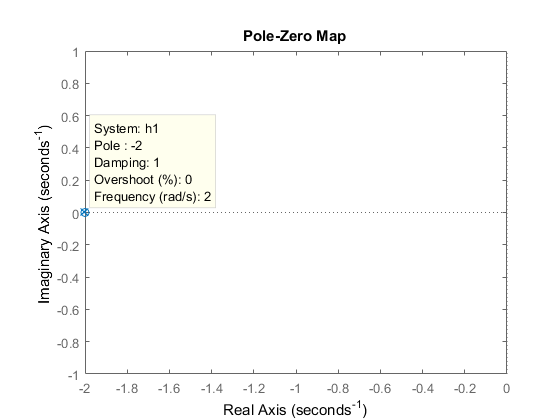
\includegraphics{img/Q1a.png}
			\caption{P\'{o}los e Zeros - Item a}	
		\end{figure}	        
		\newpage
        \subsubsection{Item b}
		\begin{figure}[!ht]
			\centering
			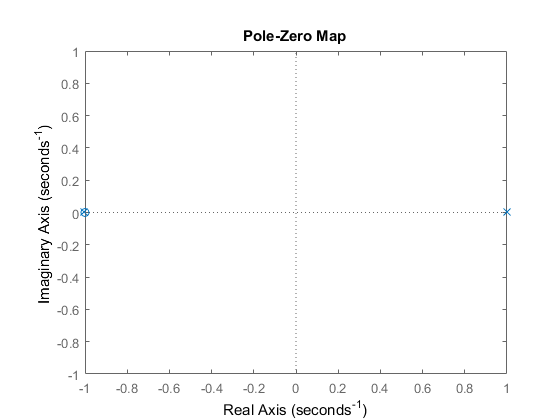
\includegraphics{img/Q1b.png}
			\caption{P\'{o}los e Zeros - Item b}	
		\end{figure}	   
		
        \[Zeros: s + 1 = 0 \rightarrow s = -1\]
        \[Polos:  s^{2} + 1 = 0 \rightarrow s = {-1; +1}\]
        \newpage
        \subsubsection{Item c}
		\begin{figure}[!ht]
			\centering
			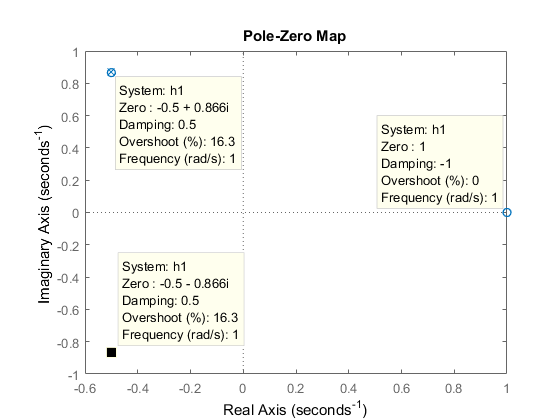
\includegraphics{img/Q1c.png}
			\caption{P\'{o}los e Zeros - Item c}	
		\end{figure}	   
		
		\[Zeros: s^{3} - 1 = 0 \rightarrow s = {\frac{-1 + \sqrt{3}}{2}; \frac{-1 - \sqrt{3}}{2}; 1}\]
		\[Polos:  s^{2} + s + 1 = 0 \rightarrow s = {\frac{-1 + \sqrt{3}}{2}; \frac{-1 - \sqrt{3}}{2}}\]        
\section{Propriedade da Transformada de Laplace}
    \subsection{Quest\~{a}o 2}
        \subsubsection{Item a}
			\[\int_{-\infty}^{+\infty} x(t-1)e^{-st}u(t)dt \rightarrow \int_{0}^{+\infty}x(\tau)e^{-s(\tau + 1)}d\tau \rightarrow e^{-s}\int_{0}^{+\infty}x(\tau)e^{-s\tau}d\tau\ \Rightarrow e^{-s}X(s)\]
        \subsubsection{Item b}
        Pela propriedade da derivação de Laplace, temos:
        \[s^3X{s} - s^2x(0^{-}) + sx^{'}(0^{-}) - x^{''}(0^{-})\]
        \subsubsection{Item c}
        Pela propriedade da integração de Laplace, temos:
        \[\frac{X(s)}{s}\]
    \subsection{Quest\~{a}o 3}
    \[\int_{-\infty}^{+\infty} cos(\omega_{0}t)u(t)e^{-st}dt \rightarrow = \frac{1}{2}\int_{0}^{\infty} e^{-t(s-\omega _{0})} + e^{-t(s+\omega _{0})}dt \rightarrow \]
    \[\frac{1}{2(s-w_{0})} + \frac{1}{2(s+w_{0})} \rightarrow \frac{s}{s^{2} + \omega _{0}^{2} } \]
\section{Resposta em Frequ\^{e}ncia}
    \subsection{Quest\~{a}o 4}
	    \[H(j\omega)  = \frac{j\omega + 2}{-\omega ^{2} + 5j\omega + 4} \]
	    \[|H(j\omega)| = \frac{\sqrt{2^{2} + {\omega ^{2}}}}{\sqrt{(4 -\omega ^{2})^{2} + (5\omega)^{2}}} \] \[\angle H(j\omega) = arctan \left(\frac{w}{2}\right) - arctan \left(\frac{5w}{4-\omega ^{2}}\right) \]
	    \[y(t) = |H(j\omega)|cos(\omega t + \phi + \angle H(j\omega))\]
        \subsubsection{Item a}
        \[y(t) = 5|H(j\omega)|cos(2t + 30^{o} + \angle H(j\omega))\]
        \[|H(j\omega)| = \frac{\sqrt{4 + 4}}{\sqrt{(4 -4)^{2} + (10)^{2}}} \Rightarrow \frac{\sqrt{2}}{5} \]
        \[\angle H(j\omega) = arctan \left(\frac{2}{2}\right) - arctan \left(\frac{10}{4-4}\right) \Rightarrow = -45^{o}\]
        \[y(t) = \sqrt{2}cos(2t -15^{o})\]
		\begin{figure}[!ht]
			\centering
			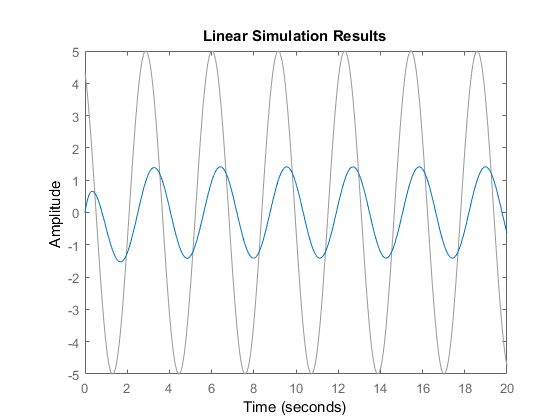
\includegraphics{img/Q4a.png}
			\caption{$y(t) = \sqrt{2}cos(2t -15^{o})$}	
		\end{figure}	         
        \subsubsection{Item b}
        \[y(t) = 10|H(j\omega)|sen(2t + 45^{o} + \angle H(j\omega))\]
        \[|H(j\omega)| = \frac{\sqrt{4 + 4}}{\sqrt{(4 -4)^{2} + (10)^{2}}} \Rightarrow \frac{\sqrt{2}}{5} \]
        \[\angle H(j\omega) = arctan \left(\frac{2}{2}\right) - arctan \left(\frac{10}{4-4}\right) \Rightarrow = -45^{o}\]
        \[y(t) = 2\sqrt{2}sen(2t)\]     
		\begin{figure}[!ht]
			\centering
			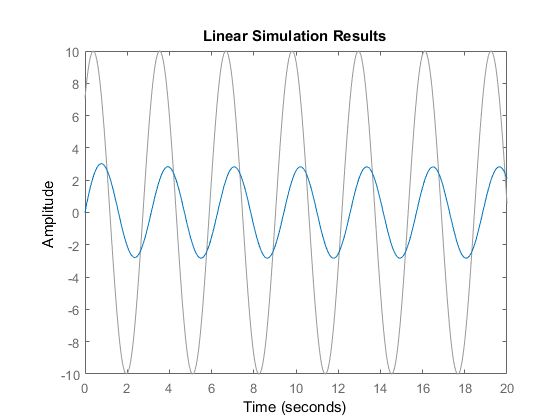
\includegraphics{img/Q4b.png}
			\caption{$y(t) = 2\sqrt{2}sen(2t)$}	
		\end{figure}	           
        \subsubsection{Item c}
        \[y(t) = 10|H(j\omega)|cos(4t + 40^{o} + \angle H(j\omega))\]
        \[|H(j\omega)| = \frac{\sqrt{4 + 16}}{\sqrt{(4 -16)^{2} + (20)^{2}}} \Rightarrow 0.2 \]
        \[\angle H(j\omega) = arctan \left(\frac{4}{2}\right) - arctan \left(\frac{20}{4-16}\right) \Rightarrow = -63.4^{o} - 59^{o} = -122.4^{o}\]
        \[y(t) = 2cos(4t -82.4^{o})\]          
		\begin{figure}[!ht]
			\centering
			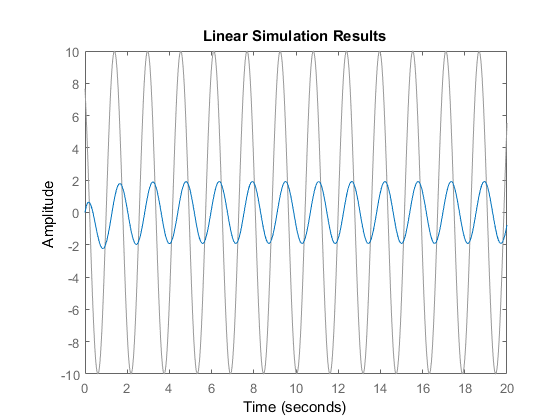
\includegraphics{img/Q4c.png}
			\caption{$y(t) = 2cos(4t -82.4^{o})$}	
		\end{figure}	        
    \subsection{Quest\~{a}o 5}
	    \[H(j\omega)  = \frac{10 - j\omega}{j\omega + 10} \]
	    \[|H(j\omega)| = \frac{\sqrt{10^{2} + {(-\omega) ^{2}}}}{\sqrt{(\omega)^{2} + (10)^{2}}} \Rightarrow 1\] 
	    \[\angle H(j\omega) = arctan \left(\frac{-w}{10}\right) - arctan \left(\frac{w}{10}\right) \]
	    \[y(t) = |H(j\omega)|cos(\omega t + \phi + \angle H(j\omega))\]   
        \subsubsection{Item a}
        \[y(t) = cos(wt + \theta + \angle H(j\omega))\]
	    \[\angle H(j\omega) = arctan \left(\frac{-w}{10}\right) - arctan \left(\frac{w}{10}\right) \]
	    \[y(t) = cos(\omega t + \theta + \angle H(j\omega))\]
	    \newpage               
        \subsubsection{Item b}
        \[y(t) = cos(2 + \theta + \angle H(j\omega))\]
        \[\angle H(j\omega) = arctan \left(\frac{-1}{10}\right) - arctan \left(\frac{1}{10}\right) \Rightarrow -11.4^{o} \]
        \[y(t) = cos(t -11.4^{o})\]    
		\begin{figure}[!ht]
			\centering
			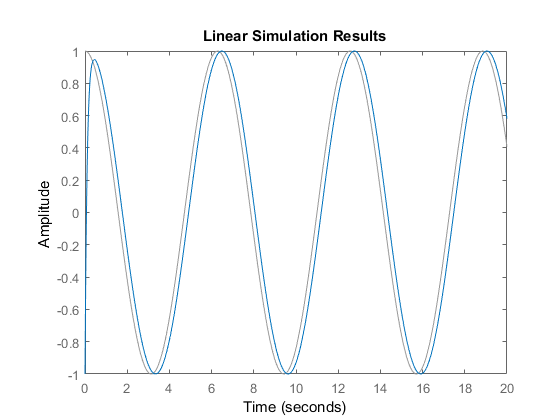
\includegraphics{img/Q5a.png}
			\caption{$y(t) = cos(t -11.4^{o})$}	
		\end{figure}	    
		\newpage                 
        \subsubsection{Item c}
        \[y(t) = cos(2t + \theta + \angle H(j\omega))\]
        \[\angle H(j\omega) = arctan \left(\frac{-2}{10}\right) - arctan \left(\frac{2}{10}\right) \Rightarrow -22.6^{o} \]
        \[y(t) = cos(2t -22.6^{o})\]   
		\begin{figure}[!ht]
			\centering
			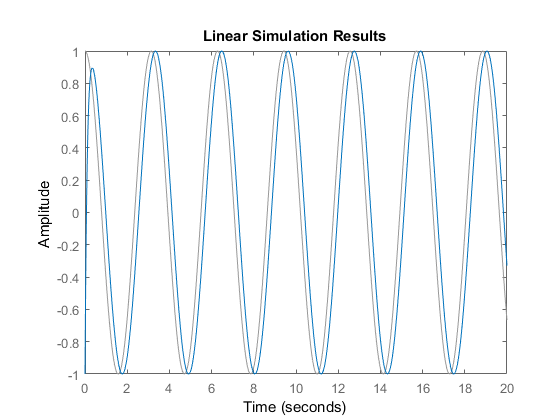
\includegraphics{img/Q5b.png}
			\caption{$y(t) = cos(2t -22.6^{o})$}	
		\end{figure}	   
		\newpage                       
        \subsubsection{Item d}
        \[y(t) = cos(10t + \theta + \angle H(j\omega))\]
        \[\angle H(j\omega) = arctan \left(\frac{-10}{10}\right) - arctan \left(\frac{10}{10}\right) \Rightarrow -22.6^{o} \]
        \[y(t) = cos(10t -90^{o})\]  
		\begin{figure}[!ht]
			\centering
			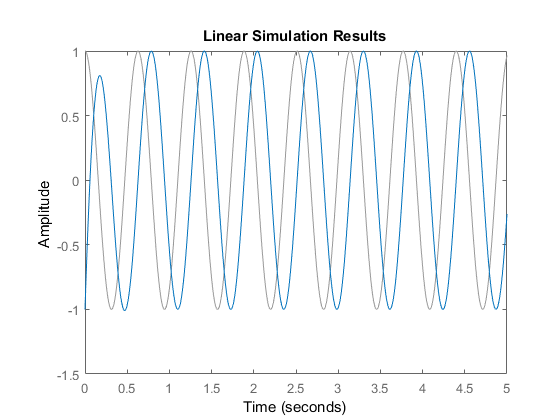
\includegraphics{img/Q5c.png}
			\caption{$y(t) = cos(10t -90^{o})$}	
		\end{figure}	       
		\newpage             
        \subsubsection{Item e}
        \[y(t) = cos(100t + \theta + \angle H(j\omega))\]
        \[\angle H(j\omega) = arctan \left(\frac{-100}{10}\right) - arctan \left(\frac{100}{10}\right) \Rightarrow -22.6^{o} \]
        \[y(t) = cos(100t -168.5^{o})\]         
		\begin{figure}[!ht]
			\centering
			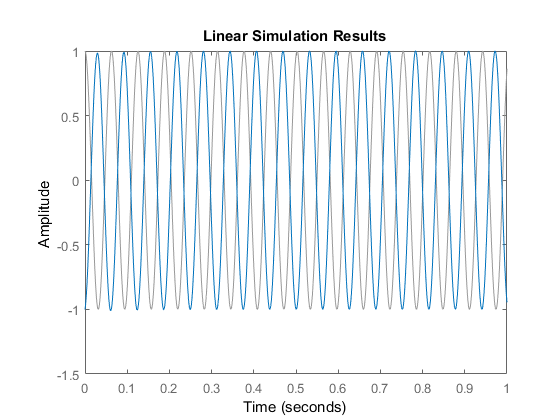
\includegraphics{img/Q5d.png}
			\caption{$y(t) = cos(100t -168.5^{o})$}	
		\end{figure}	           
    \subsection{Quest\~{a}o 6}
        \subsubsection{Item a}
        É possível, uma vez que a resposta e um deslocamento de fase.
        \subsubsection{Item b}
        Não é possível, uma vez que ocorre uma alteração na frequência.
        \subsubsection{Item c}
        É possível, o sinal de saída e o mesmo que a entrada.
\section{Diagrama de Bode}
    \subsection{Quest\~{a}o 7}
        \subsubsection{Item a}
		\begin{figure}[!ht]
			\centering
			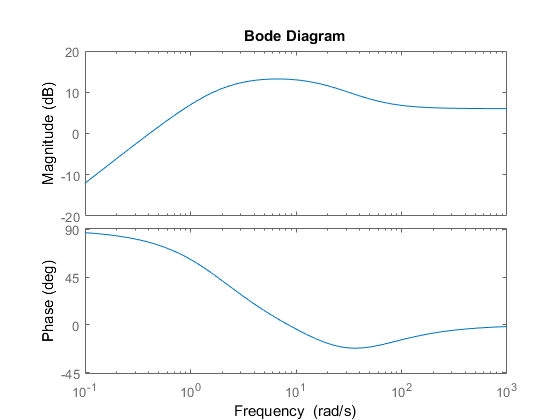
\includegraphics{img/Q7a.png}
			\caption{Diagrama de Bode - Item a}	
		\end{figure}	       
		\newpage 
        \subsubsection{Item b}
		\begin{figure}[!ht]
			\centering
			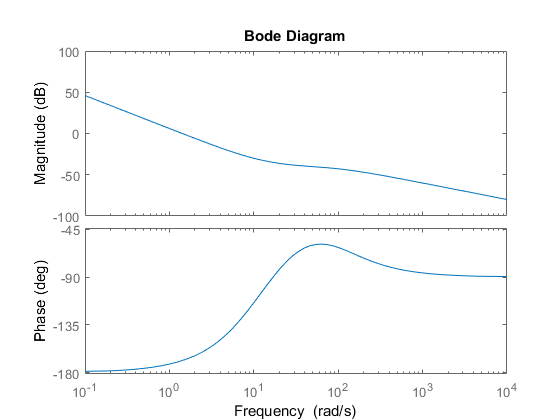
\includegraphics{img/Q7b.png}
			\caption{Diagrama de Bode - Item b}	
		\end{figure}       
		\newpage
        \subsubsection{Item c}
		\begin{figure}[!ht]
			\centering
			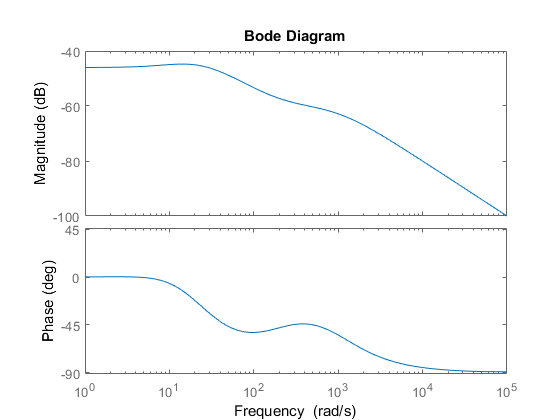
\includegraphics{img/Q7c.png}
			\caption{Diagrama de Bode - Item c}	
		\end{figure}         
		\newpage
        \subsubsection{Item d}
		\begin{figure}[!ht]
			\centering
			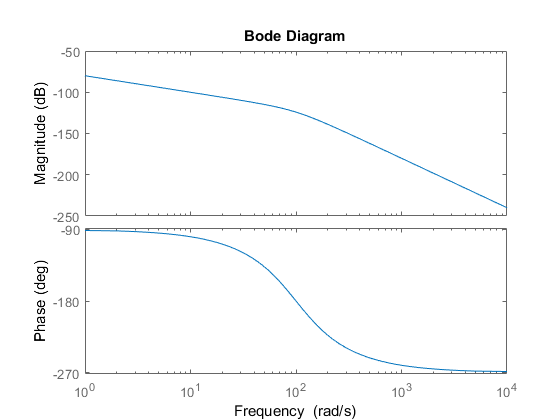
\includegraphics{img/Q7d.png}
			\caption{Diagrama de Bode - Item d}	
		\end{figure}          
	\newpage   
    \subsection{Quest\~{a}o 8}
        \subsubsection{Item a}
		\begin{figure}[!ht]
			\centering
			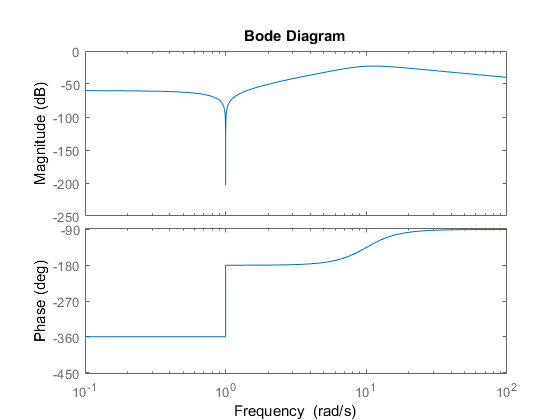
\includegraphics{img/Q8a.png}
			\caption{Diagrama de Bode - Item a}	
		\end{figure}           
		Nenhuma das figuras disponibilizadas.
		\newpage
        \subsubsection{Item b}
		\begin{figure}[!ht]
			\centering
			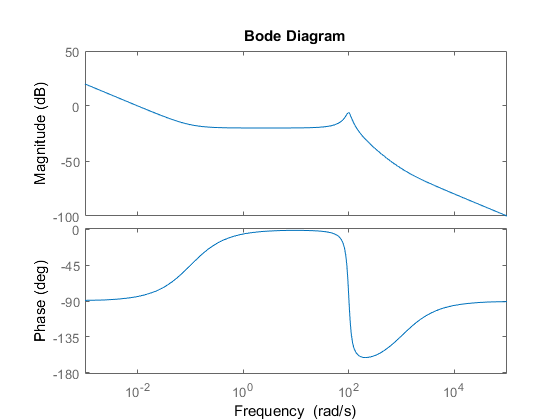
\includegraphics{img/Q8b.png}
			\caption{Diagrama de Bode - Item b}	
		\end{figure}           
		Resposta: \textbf{Figura 2}
		\newpage
        \subsubsection{Item c}
		\begin{figure}[!ht]
			\centering
			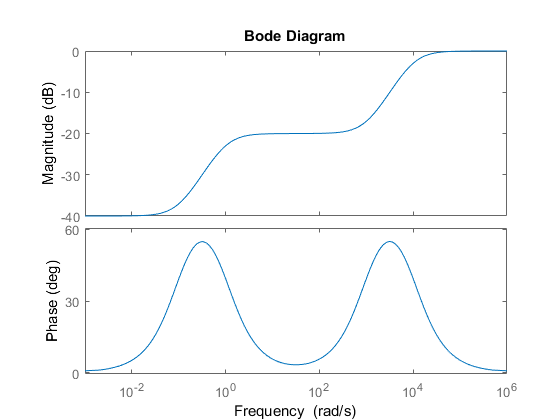
\includegraphics{img/Q8c.png}
			\caption{Diagrama de Bode - Item c}	
		\end{figure}           
		Resposta: \textbf{Figura 1} 
		\newpage         
        \subsubsection{Item d}
		\begin{figure}[!ht]
			\centering
			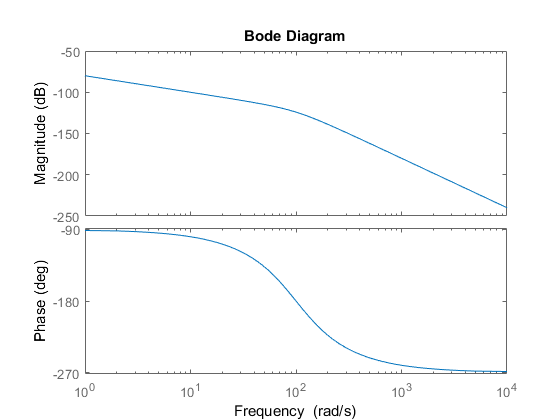
\includegraphics{img/Q8d.png}
			\caption{Diagrama de Bode - Item d}	
		\end{figure}           
		Resposta: \textbf{Figura 3}        
\end{document}